\documentclass[11pt,a4paper]{article}
\usepackage[dutch]{babel}
\usepackage{graphicx}
%\usepackage[final]{graphicx}
\usepackage{subcaption}
\usepackage{epstopdf}
\usepackage{amsmath}
\usepackage{amssymb}
\usepackage{url}
\usepackage{fixltx2e}
%\usepackage[numbered]{mcode}
\usepackage{listings}
\usepackage[margin=1.1in]{geometry}
\usepackage[retainorgcmds]{IEEEtrantools}
\usepackage{hyperref}
\usepackage{cleveref}
\usepackage{xcolor}

\setlength\parindent{0pt}

\begin{document}

\begin{center}
\section*{Millieuvriendelijke oplaadpunten voor e-bikes}
\end{center}
In een groep met 6 bachelorstudenten van de TU Delft zijn wij bezig met het ontwikkelen van een fictief businessplan. In het kader van het marktonderzoek heeft u dit bestand ontvangen. Hieronder staat puntsgewijs wat het concept inhoudt. Onder aan de pagina kunt u een grafische weergave van het concept vinden.\\

Het idee:
\begin{itemize}
\item Gratis opladen bij groene/millieubewuste oplaadpunten met zonnepanelen voor e-bikes
\item Eveneens oplaadpunten voor telefoons en gratis WiFi bij het oplaadpunt
\item Een bijbehorende app en website waarmee gebruikers een plaats kunnen reserveren en de status van hun fiets kunnen bekijken
\item Geen aanschafkosten voor de gemeente, alleen het beschikbaar stellen van ruimte en een electriciteitsaansluiting
\item Batterijen in het oplaadpunt voor optimale continu\"iteit van de de stroomvoorziening
\item De ruimte die nodig is om het oplaadpunt te plaatsen is slechts enkele vierkante meter
\item Middels advertenties van bedrijven in de app en op de website worden de oplaadpunten voor het bedrijf rendabel

\end{itemize}

Wat wij graag zouden willen weten:
\begin{itemize}
\item Zijn er in uw gemeente initiatieven en/of plannen om groene oplaadpalen te plaatsen?
\item Denkt u dat er vanuit de gemeente interesse zou zijn om deze oplaadpunten te plaatsen? 
\end{itemize}

Wij zouden het erg op prijs stellen als u op deze vragen zou kunnen reageren.\\
Hartelijk dank!\\\\

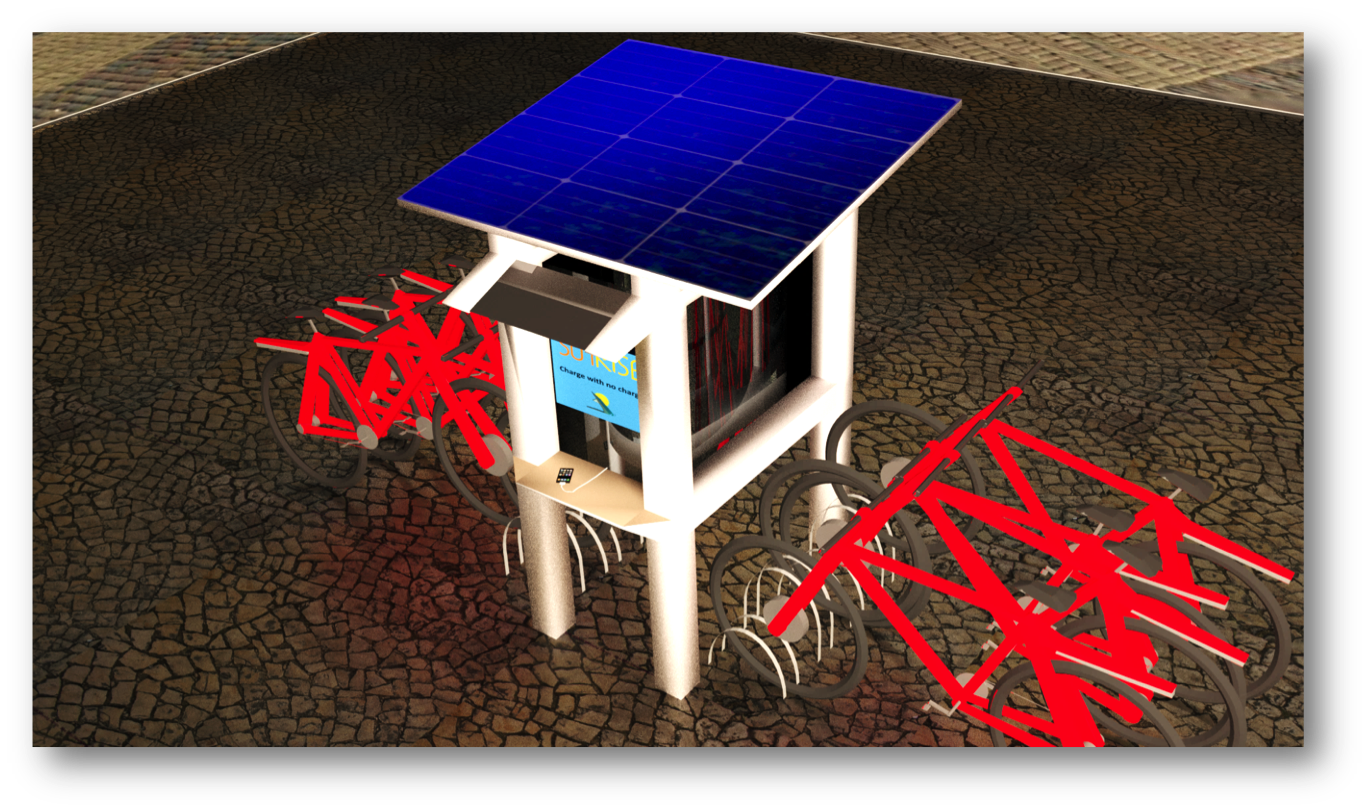
\includegraphics[width=\textwidth]{render2.png}

\thispagestyle{empty}
\end{document}